\documentclass{article}
\usepackage[english]{babel}
\usepackage[utf8]{inputenc}
\usepackage{graphicx}
\usepackage{caption}
\usepackage{float}
\usepackage[normalem]{ulem}
\useunder{\uline}{\ul}{}
\usepackage{rotating}
\usepackage{gensymb}
\usepackage{tikz}
\linespread{1.46}
\usepackage[
    top=3cm,
    bottom=3cm,
    left=3cm,
    right=3cm,
]{geometry}

\begin{document}

\title{Master Thesis Summary: \textit{Development, Test and Application of a framework for cloud serverless services}}

\author{Andrea Santu [s251579]}

\maketitle

\section{Introduction}
The overview of services for the creation of Web Applications is focusing more
and more towards a micro services oriented approach, moving away from monolithic
structures.
The maximum representation of this is with the serverless paradigm, which has
found an implementation in the cloud model Function as a Service (FaaS), a model
that uses plain simple functions as its main resources.
The provisioning model of traditional servers is based on renting server space, which
is generally over-purchased, to ensure handling spikes in the number of incoming
http(s) requests (internet requests).
The FaaS model differs from the latter as each function is executed and billed
only in response to an event, obtaining a fine grained usage of the physical
infrastructure and paying on an as-used basis.
In the context of Web Applications an event could be a network event (e.g. http
requests), a timer event (either one-shot or interval) or other customized trigger
event.
The main advantages of this model are:
1) Simplified development and deployment process. The first one is due to the fact that
the code is splitted into simple independent functions, each one with a defined purpose.
The latter is improved because each function can be deployed singularly, cutting
the time needed to provide fixes for bugs and critical issues.
2) The service is auto-scaling, so based on the server load (e.g. the number of
received internet requests) the cloud provider takes care of creating new instances
of the required functions.
3) Cost effective as only function execution is billed, opposing to the traditional
approach where also idle time is included in the cost.

\noindent
Serverless Framework has emerged as one of the major framework that allows the
usage of the homonym paradigm in a simple way.
Despite the functionalities introduced by Serverless, the developer must take
charge of various operations concerning indirectly the business logic of the
application.
The proposed framework, named \textit{Restlessness}, was born with the goal of
improving the user experience of Serverless, providing a standard project and testing
structure, a Command Line Interface and a local Web Interface through which is
possible to completely manage the project and with the further goal of minimizing
all operations that do not concern directly the application's business logic.

\section{Methodology}
The main goal of the thesis has been to develop the framework from its initial and
barely usable implementation, to a software that can be used without problems on
real deployed web applications.

\noindent
Part of the development has been spent on creating a productive development
workflow, with tools for Continuous Integration and Continuous Delivery, provided
by the CircleCi platform and a version control system, provided by the Github
platform.
The project has then been splitted into two main components, corresponding to the
packages provided on the Npm registry\footnote{The Node package Manager, it allows
publishing and installing Node.js packages}: \mbox{\textit{@restlessness/cli}} and
\mbox{\textit{@restlessness/core}}.

\noindent
The \textit{core} package has been developed firstly, as it defines the structure
that a newly created \textit{Restlessness} project should have, and also provides
all classes and functions allowing the management of the project at a low level,
such as the interaction with it on the file system. The management of the project
includes the creation of serverless resources, with the main ones being: Endpoints
and Schedules, corresponding to serverless functions executed in response to http
and periodic or programmed events respectively; Authorizers, functions that perform
authorization operation, granting or denying access to functions or other resources;
Models: classes modeling resources, primarily database objects; Services, a group
of serverless functions.

\noindent
The latter package is composed by a Command Line Interface and a local Web Interface,
providing the main interaction points for the user, and it rely on the \textit{core}
package to provides its functionalities. The local Web Interface is composed by
a frontend and backend application, with the latter created with the framework
itself, primarily for the advantage of a simplified development.
All togheter those components allow: to create a project, to develop it locally
and deploying it on the cloud provider platform.

\noindent
The framework has been designed to be extended by external addons packages, so the
next step in the development process has been to provide addons for common patterns,
such as database access and authentication. This has been done through the packages
\mbox{\textit{@restlessness/dao-mongo}} and \mbox{\textit{@restlessness/auth-jwt}},
respectively for interaction with the mongodb database and for authentication through
the Json Web Token standard.

\begin{figure}[h]
    \centering
    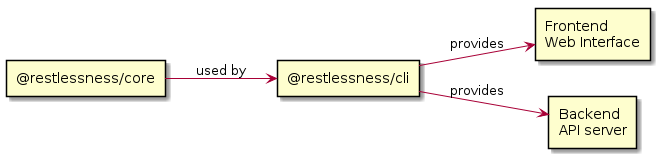
\includegraphics[width=12cm]{../source/diagrams/rln_components.png}
    \caption{Restlessness main components}
\end{figure}

\section{Application}
It has been possible to test the developed framework on real deployed applications,
thus allowing to find and correct critical issues. The main test case has been the
implementation of the backend application for the project \textit{Spazio alla Scuola},
which is a platform thought by the \textit{Fondazione Agnelli}, a non-profit
foundation born in 1966 in Turin.
The aim of the project was to provide a concrete support to school leaders for lecture
resumption on September 2020, given the health situation on the coutry due to the
SARS-CoV-2 pandemic. The platform, provided as a free service, offers tools to
verify the capacity of classrooms and other school spaces, to plan classrooms flows
and staggering, in compliance with the distancing measures.
The serverless approach, used in conjunction with the \textit{Restlessness} framework,
is suited in this particular case because: the number of http(s) requests through the
day is variable; the project requires a fast development, so having a framework
already providing a project structure and solution for common patterns simplify
this process.

\noindent
The proposed framework provided the speed of development sought, however, due to
its early stage of development, some problems arised.
In particular the main improvements that have been made to the framework after the
application on \textit{Spazio alla Scuola} are: handling of Cold start, which is
a delay in the function execution due to initialization operations needed by the
cloud provider; creation of a plugin to support the non relational database mongodb
in a serverless context, and in particular to avoid the saturation of available
database connections; support of multiple services under a single
\textit{Restlessness} project.

\noindent
Addressing those problems led the \textit{Restlessness} framework to be more stable
and reliable, both for the described project, being it able to handle 500 thousand
requests at its peak and also for other production applications, where it is currently
used.

\section{Conclusions}
At the end of this development cycle, the proposed framework has become production
ready, however, its development is not completed and the main improvements on its
roadmap are: becoming framework agnostic, while at the moment the only supported
provider is AWS; proposing a structure for integration testing; integrate all Cli
functionalities on the Web Interface and vice versa, to achieve greater flexibily;
to provide additional extensions to extend the framework usability.

\end{document}
